\documentclass[12pt]{article}
\usepackage{xeCJK}
\setCJKmainfont{SimSong} 
\usepackage{amsmath, amssymb, bm}
\usepackage{fancyhdr}
\usepackage{graphicx}
\usepackage{listings}
\usepackage{xcolor}
\usepackage{caption}
\usepackage{float}
\usepackage{pythonhighlight}

\definecolor{codegray}{rgb}{0.95,0.95,0.95}
\lstset{
    backgroundcolor=\color{codegray},
    basicstyle=\ttfamily\footnotesize,
    breaklines=true,
    frame=single,
    language=Python,
    keywordstyle=\color{blue},
    commentstyle=\color{gray},
    stringstyle=\color{green!50!black},
    showstringspaces=false
}

\title{一维交替质量弹簧链的振动模态分析}
\author{231503031 汤轶文}
\date{\today}

\begin{document}

\maketitle

\section{问题背景}

在固体物理中,晶格的振动行为对材料的热学、光学和声学性质具有重要影响。本文研究一维交替质量的弹簧-小球系统中正常模的振动特性,该模型可类比于实际晶格中的声子色散关系,并展示了声学支与光学支的分离。

\section{物理建模与理论推导}

我们考虑一维弹簧链系统,由质量交替为 $m_1$ 和 $m_2$ 的 $N$ 个小球组成,相邻小球由劲度系数为 $k$ 的弹簧连接,忽略阻尼。

系统的势能可以写为:
\[
V = \frac{k}{2} \sum_{i=1}^{N-1} (x_{i+1} - x_i)^2
\]

引入 $N \times N$ 的刚度矩阵 $K$,其形式为三对角矩阵:
\[
K = \begin{bmatrix}
2 & -1 & 0 & \cdots & 0 \\
-1 & 2 & -1 & \ddots & \vdots \\
0 & -1 & \ddots & \ddots & 0 \\
\vdots & \ddots & \ddots & 2 & -1 \\
0 & \cdots & 0 & -1 & 2
\end{bmatrix}
\]

质量矩阵为对角矩阵 $M = \text{diag}(m_1, m_2, m_1, m_2, \dots)$。牛顿第二定律写为矩阵形式:
\[
M \ddot{\bm{x}} + K \bm{x} = 0
\]

令 $\bm{x}(t) = \bm{u} e^{i \omega t}$,代入上式得广义特征值问题:
\[
K \bm{u} = \omega^2 M \bm{u}
\]

\section{数值实现}

我们采用 Python 实现上述模型,对 $A = M^{-1}K$ 进行对角化,获得系统的本征频率 $\omega$ 和模态 $\bm{u}$。

\subsection*{主要参数设置}

\begin{itemize}
  \item 质量 $m_1 = 1.0$, $m_2 = 2.0$
  \item 弹簧劲度系数 $k = 1.0$
  \item 系统粒子数 $N = 100$
\end{itemize}

\subsection*{关键代码}

\begin{python}
import numpy as np
import matplotlib.pyplot as plt

N = 100
k = 1.0
m1 = 1.0
m2 = 2.0

K = 2*np.eye(N) - np.eye(N, 1) - np.eye(N, -1)
masses = np.array([m1 if i % 2 == 0 else m2 for i in range(N)])
M = np.diag(masses)
A = np.linalg.inv(M) @ K
omega2, modes = np.linalg.eigh(A)
omega = np.sqrt(omega2)
\end{python}

我们对前 $N/2$ 个模态作为声学支,其余作为光学支,并与波矢 $q$ 建立对应关系:
\[
q_n = \frac{n\pi}{N/2 + 1}, \quad n = 1,2,\dots,N/2
\]

\section{计算结果与分析}

\begin{figure}[H]
    \centering
    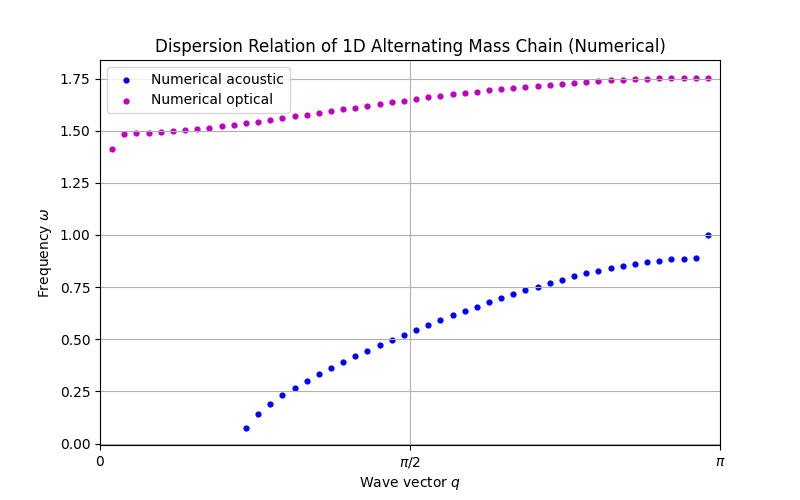
\includegraphics[width=0.7\textwidth]{dispersion.png}
    \caption{交替质量弹簧链的色散关系}
\end{figure}

从图中可以观察到:

\begin{itemize}
    \item 声学支(蓝色)频率从 0 单调上升,表现为系统整体平移和低频振动模;
    \item 光学支(紫色)频率较高,表现为相邻质量反向振动;
    \item 色散关系呈非线性,符合实际晶格动力学中双原子链模型的结果。
\end{itemize}

\section{结论}

本研究数值求解了一维交替质量弹簧链的正常模问题。通过对 $M^{-1}K$ 进行对角化,成功获得系统的声学支与光学支振动模态和对应频率。结果验证了交替质量对声子色散关系的显著影响,可为理解固体物理中的晶格动力学行为提供基础模型支持。

\section*{附录:完整程序}

\begin{lstlisting}
import numpy as np
import matplotlib.pyplot as plt

N = 100
k = 1.0
m1 = 1.0
m2 = 2.0

K = 2*np.eye(N) - np.eye(N, k=1) - np.eye(N, k=-1)
masses = np.array([m1 if i % 2 == 0 else m2 for i in range(N)])
M = np.diag(masses)
A = np.linalg.inv(M) @ K
omega2, modes = np.linalg.eigh(A)
omega = np.sqrt(omega2)

q_vals = np.arange(1, N//2+1) * np.pi / (N//2 + 1)

omega_ac = omega[:N//2]
omega_op = omega[N//2:N]

plt.figure(figsize=(8,5))
plt.scatter(q_vals, omega_ac, c='b', s=12, label='Numerical acoustic')
plt.scatter(q_vals, omega_op, c='m', s=12, label='Numerical optical')
plt.xlabel("Wave vector $q$")
plt.ylabel("Frequency $\omega$")
plt.title("Dispersion Relation of 1D Alternating Mass Chain (Numerical)")
plt.grid()
plt.xlim(0, np.pi)
plt.xticks([0, np.pi/2, np.pi], ["0", r"$\pi/2$", r"$\pi$"])
plt.legend()
plt.savefig("dispersion.png")
plt.show()
\end{lstlisting}

\end{document}